\section{Preliminary}
This experiment uses answers from HELM set, which is collected from 183 test-takers on 22 datasets. This creates a response matrix with size $183 \times 78712$. Each dataset is assumed to test a small subset of predetermined skills ($n\le 3$) based on their description. 

There should be a significant overlap of skills for every dataset (specialised upstream task) as is present with the common consensus for the generalisation of many standardised exams. To verify this claim, I have conducted some preliminary data analysis.
\subsection{Correlation metrics}
The probability of correct answers shows significant correlations, as is present in Fig.1. This prompted the first Principal Component Analysis (PCA) on the dataset. I started with the first number of dimensions that begins to show a significant variance ($\sigma^2\ge 95\%$), arriving at $\dim=7$. Further analysis of PC loadings has led to a reasonable interpretation of each PC based on influential datasets.
\begin{itemize}
    \item [--] PC1: Foundational vs. Expert Reasoning
    \item [--] PC2: General Academic Aptitude
    \item [--] PC3: Thai-Specific Proficiency
    \item [--] PC4: Thai Benchmark Conflict
    \item [--] PC5: Safety vs. Specificity Trade-off
    \item [--] PC6: Abstract vs. Applied Language Reasoning
    \item [--] PC7: MMLU Specialization
\end{itemize}

I only considered datasets with significant influence ($|\text{load}| \ge 0.4$) for interpretation. Note that these are only suggested names for easy reference; further analysis is needed to understand specific PCs. The full loading result is attached in Appendix A of this report. This resulted in 6 meaningful PCs (PC1 didn't have a significant-load dataset).

\begin{figure}[!t]
    \centering
    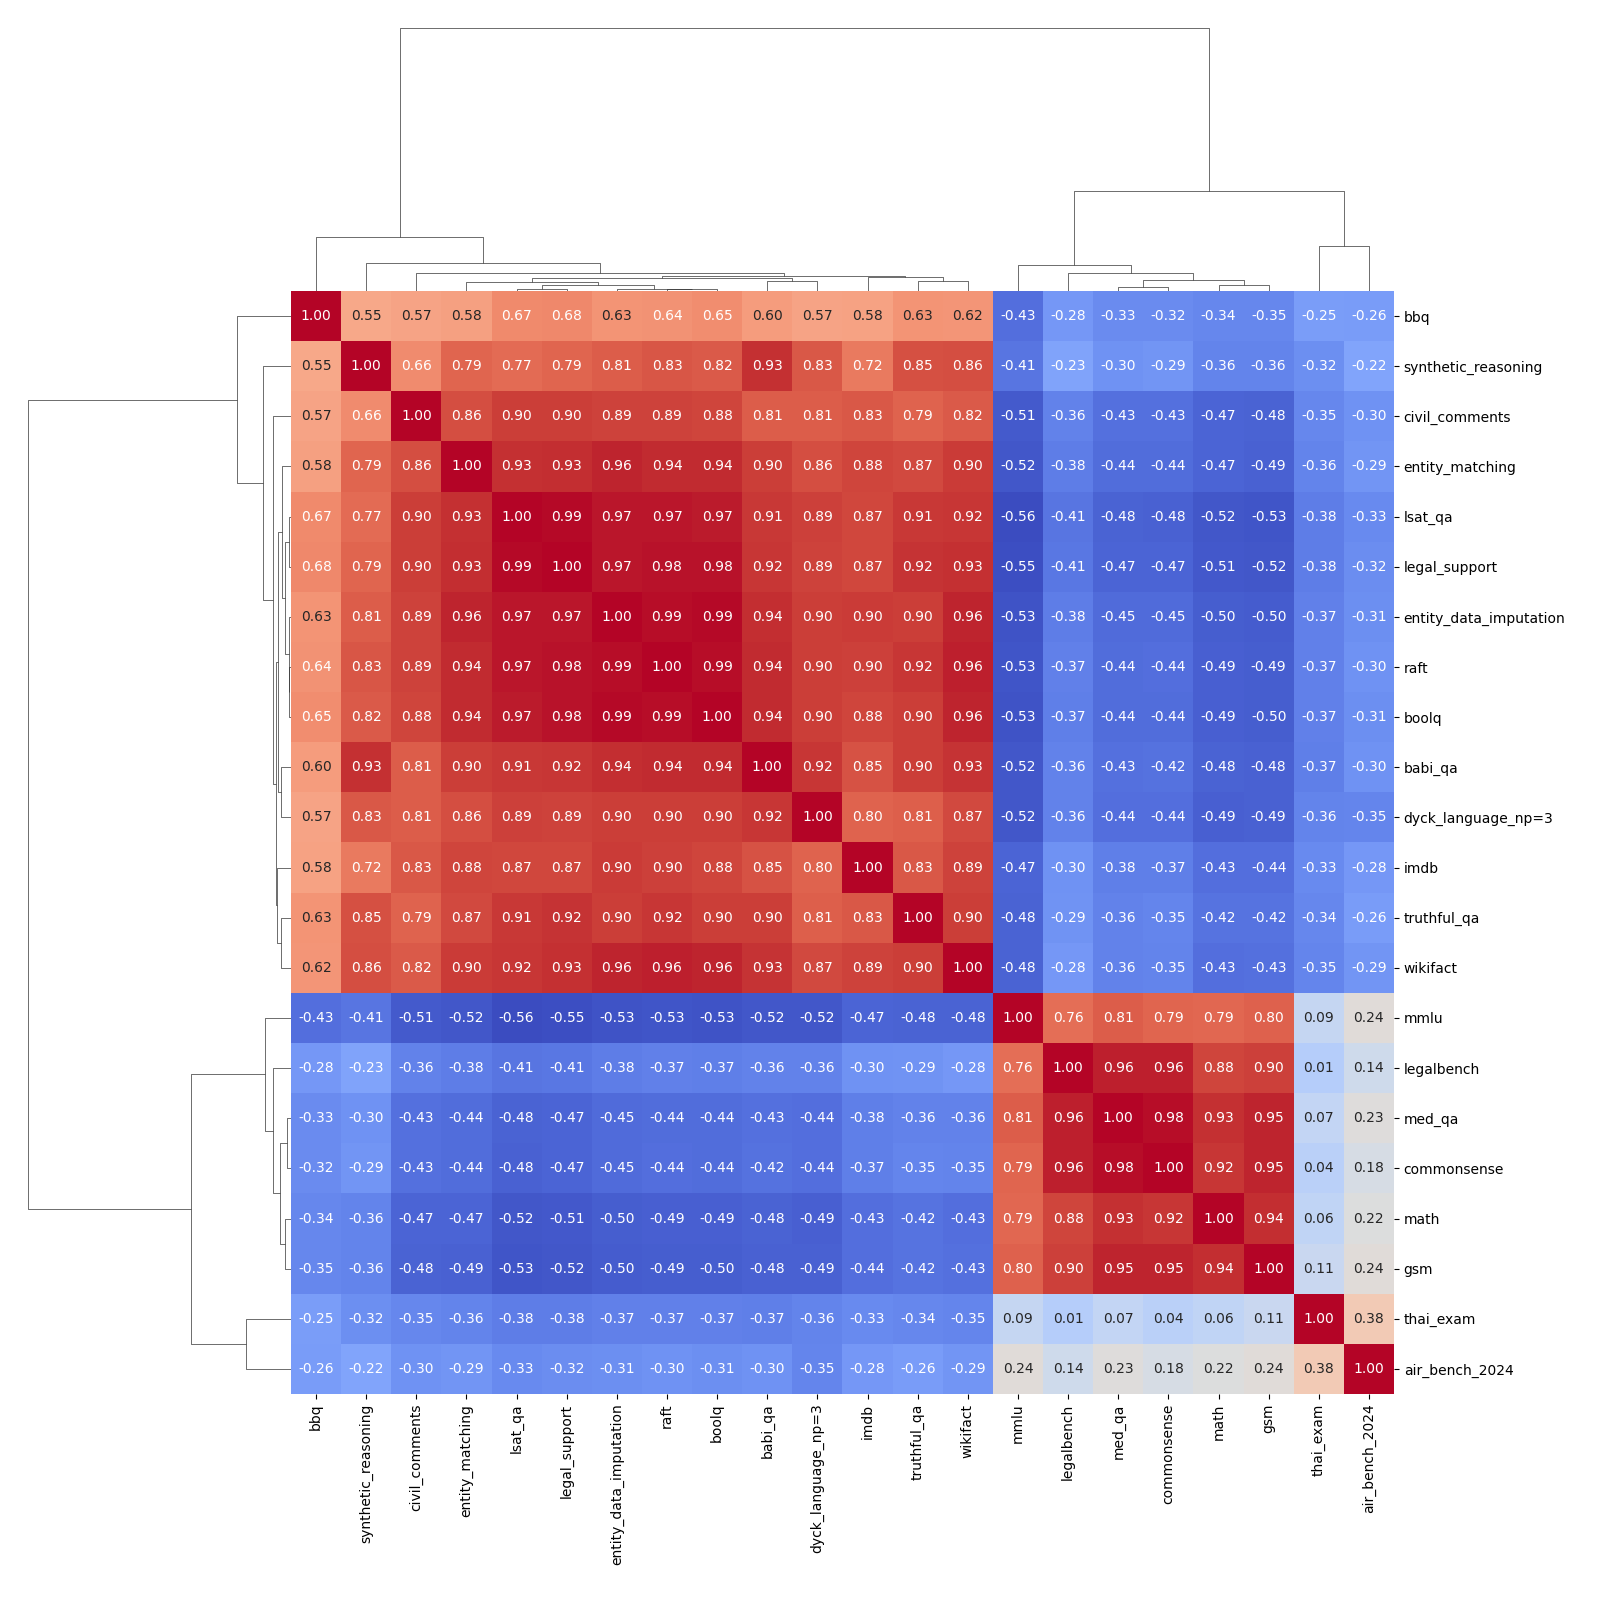
\includegraphics[height=\linewidth]{figures/resmat_corr_scenario.png}
    \caption{Clustered Correlation Matrix Heatmap for the probability of correct in each dataset.}
    \label{fig:resmat_corr_scenario}
\end{figure}

\subsection{Factor analysis}

I also performed an additional factor analysis to verify the reliability of my PCA. I performed orthogonal rotation on different number of dimensions and found that both 7 and 9 number of PC yields the most AUC and Pearson Correlation, very close to the 2-PL model. However, when testing for strongest loaders, the results in each dimension are identical, indicating the data may have a strong global factor that overshadows more subtle, distinct latent traits.
